\documentclass{llncs}
\pagestyle{plain}
%\usepackage[margin=2.5cm]{geometry}
\usepackage[pdftex]{graphicx}
\usepackage{caption}
\usepackage{subcaption}
\usepackage[rightcaption]{sidecap}
\usepackage{float}
\usepackage[ruled, vlined, linesnumbered]{algorithm2e}
\SetAlgoSkip{bigskip}
\usepackage{hyperref}
\usepackage{amsmath}
\usepackage{titling}
\usepackage{soul}
\usepackage{cite}

\usepackage{fancyhdr}
\pagestyle{fancy}
\fancyhf{}
\lhead{Seminar: Recent Results in Swarm Intelligence}
\rhead{Winter 2014/15}
\cfoot{\thepage}

\setlength{\droptitle}{-4em}
\title{Search Improvemnt Based on Ants Performance in Image Edge Detection using ACO}
\author{Syam Ajay Simha Gullipalli\\
		Universit\"at Paderborn\\
		\texttt{syam@mail.uni-paderborn.de}}
\date{\today}

\begin{document}
	\maketitle
	\thispagestyle{fancy}
	
	\begin{abstract}
	Ant Colony Optimization (ACO) is a popular metaheuristic framework used to solve diverse combinatorial optimization problems. Graph problems can be seen as combinatorial optimization problems which could be solved using ACO algorithms. Image edge detection is already attained through ACO algorithms by representing image as graph. The existing mehods leave noise on the resultant image which is reduced through thresholding by attempting different threshold values. The proposed thecnique leads the ants towards good solutions based on the average performance of ants which does not require reduction of noise.
	\end{abstract}
	
	\begin{keywords}
	Ant Colony Optimization, Edge Detection, Ant Colony System, Image Processing.
	\end{keywords}
	
	\section{Introduction} \label{sec:introduction}
	Edge Detection is one of the early stages of machine vision applications, which is used to estimate structural features of a given image. The edges in an image are determined by finding abrupt changes in intensity levels of neighbor pixels. The conventional edge detecion methods use smoothing functions to reduce the noise, and complex mathematical functions like first and second order derivatices and thresholding techniques to find edges. These methods may fail to find all possible edges. Edge detection using Ant Colony Optimization (ACO) algorithm may dominate the conventional edge detection methods, because it takes the advantage of a number of ants to find partial solutions, and these partial solutions are collectively used to produce complete possible solution. 
	
	ACO is a population based metaheuristc which is inspispred by the foraging behavior of ants \cite{Dorigo:2004, Dorigo:2007, Blum:2005}.  A number of ACO-based algorithms have been developed since Dorigo et al. first proposed in early 1990's. Ant System (AS) is the first algorithm which is the base for other varants. Rank-based Ant System (RAS), Max-Min Ant System (MMAS), Elitist Ant System (EAS), Ant Colony System (ACS) are the successors of AS in which the main difference lies in how the pheromone is updated \cite{Dorigo:2004, Dorigo:2007}. The proposed technique uses ACS which benefits from the two levels of pheromone update.

	The image should be transformed into a graph representing a set of vertices and edges. Then ACO algorithm is applied on the resulting graph to construct pheromone matrix. Section \ref{sec:soa_edge_detection} describes how the image is transformed and some state-of-the-art algorithms using ACO to find edges using the transformed graph. The proposed technique, how initialization of ants effect the results is expalined in section \ref{sec:imp_search}. The results of the proposed technique are analyzed in section \ref{sec:comparision}.
	
	\section{State-of-the-art Algorithms for Edge Detection} \label{sec:soa_edge_detection}
	Many experiments show that the ACO metaheuristic could be successfully used to find edges in an image. Edge detection using the transition and pheromone update rules of AS are presented in literature \cite{Alirezae:2008}. Many experiments prove that the ACS variant dominates AS in edge detection \cite{Anna:2010,Agarwal:2012,Jian:2012} because of it's two levels of pheromone update (local and global). A hybrid edge detection using Canny edge detector and ACS is presented in literature \cite{Manish:2013}, and edge  detection using quantam computing and ACS is presented in literature \cite{Jian:2012} which use complex mathematical functions like matrix multiplications and trignometric functions. The proposed technique does not use those complex functions. Instead, it extends the work presented in literature \cite{Anna:2010}. In order to apply ACS on an image, it should be transformed into a graph. Therefore, a matrix $I_{w\times h}$ representing the intensity at each pixel is constructed as shown in figure \ref{fig:ImageGraph}.
	
	%FIGURE: Image Graph
	\begin{SCfigure}
		\centering
		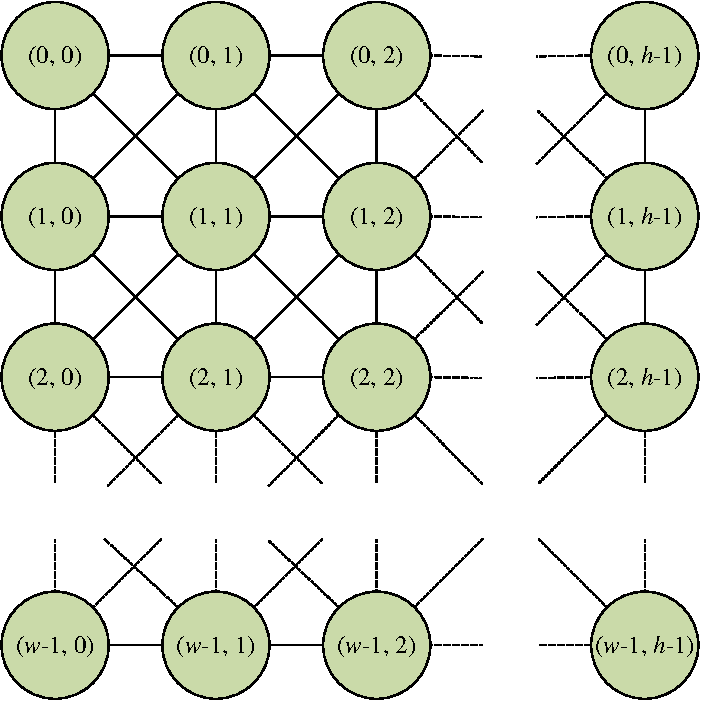
\includegraphics[width=0.35\textwidth]{IMG/GraphImage}
		\caption{Graph representation of $w\times h$ image. Each pixel in the image is considered as a node and each node is connected to its neighbors (horizontal, vertical, and diagonal) to form edges. \cite{Anna:2010}}
		\label{fig:ImageGraph}
	\end{SCfigure}
	
	The pseudocode for edge detection using ACS is as shown in algorithm \ref{alg:aco}. $K$ artificial ants are randomly distributed over the image and their movements are guided by the variation in pixel intensity levels.
	
	\begin{algorithm}
		Initialization\;
		\ForAll{iterations n in 1:N}{
			\ForAll{construction steps l in 1:L}{
				\ForAll{ants k in 1:K}{
					Choose and move to the next pixel\;
					Update local pheromone\;
				}
			}
			Update global pheromone values on visited pixels\;
		}
	\caption{Pseudocode for edge detection using ACS.\cite{Anna:2010}}\label{alg:aco}
	\end{algorithm}
	
	In the initialization step all the values in pheromone matrix are set to a constant $\tau_{0}$ (usually small but not zero). An exploitation paramerter $q_0$, a constant between 0 and 1 is given. At each construction step every ant moves from it's current pixel to it's neighborhood pixel based on a random number $q$ uniformly distributed between 0 and 1, using pseudorandom proportional rule as shown in equation \eqref{eq:acs}.
	
	\begin{equation}
		\centering
		j = \left\{
		\begin{array}{l l}
		\text{arg max}_{j \in N_i^k} (\tau_{ij}^{\alpha} \cdot \eta_{ij}^{\beta}) & \quad \text{if } q \leq q_0 \text{(Exploitation)}\\
		J & \quad \text{otherwise (Exploration)}
		\end{array} \right.
		\label{eq:acs}
	\end{equation}
	
	Where $N_i^k$ is the set of unvisited neighbors and $J$ is selected using trasition probability rule as in equation \eqref{eq:tp}.
	
	\begin{equation}
		\centering
		p^{(k)}_{ij}(t)  = \frac{[\tau_{ij}(t)]^\alpha[\eta_{ij}]^\beta}
		{\sum_{l \in N_i^k} [\tau_{il}(t)]^\alpha [\eta_{il}]^\beta}
		\label{eq:tp}
	\end{equation}
	
	$\tau_{ij}$ is the pheromone value and $\eta_{ij}$ is the heuristic information at pixel ($i$, $j$) which are influenced by constants $\alpha$ and $\beta$ respectively. $\eta_{ij}$ is calculated as in equation \eqref{eq:heuristic}.
	
	\begin{equation}
		\eta_{ij} = \frac{V_c(I_{ij})}{V_{max}}
		\label{eq:heuristic}
	\end{equation}
	
	$I_{ij}$ is the intensity of pixel ($i$, $j$). $V_c(I_{ij})$ is the function (equation \eqref{eq:intensity}) of intensity variation around the pixel ($i$, $j$) as shown in figure \ref{fig:pixelConf}. $V_{max}$ is the maximum intensity variation in given image.
	
	\begin{align}
		\centering
		V_c(I_{(i, j)}) &= |I_{(i-1, j-1)} - I_{(i+1, j+1)}| + |I_{(i, j-1)} - I_{(i, j+1)}| \nonumber \\
		&\qquad + |I_{(i+1, j-1)} - I_{(i-1, j+1)}| + |I_{(i+1, j)} - I_{(i-1, j)}|
		\label{eq:intensity}
	\end{align}
	
	\begin{figure}[H]
		\centering
		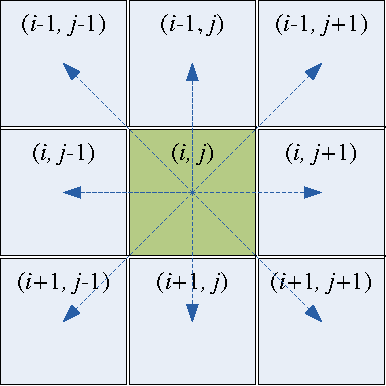
\includegraphics[width=0.25\textwidth]{IMG/NeighboringPixels}
		\caption{Computing intensity variation at pixel ($i$, $j$). \cite{Anna:2010}}
		\label{fig:pixelConf}
	\end{figure}

	At each move ants update the local pheromone value of the visited pixel as in equation \eqref{eq:localupdate}. $\varphi$ is the pheromone decay coefficient. Repeated visit of same set of nodes by an ant is restricted by maintaining a memory at each ant. 
	
	\begin{equation}
		\centering
		\tau_{ij} \leftarrow (1 - \varphi) \cdot \tau_{ij} + \varphi \cdot \tau_{0}
		\label{eq:localupdate}
	\end{equation}
	
	After each construction step, global pheromone is updated on visited pixels using equation \eqref{eq:globalupdate}. $\rho$ is the pheromone evaporation coefficient in range (0, 1]. $\Delta \tau^{k}_{ij}$ is the amount of pheromone updated by ant k on pixel ($i$, $j$). If ant k visited pixel ($i$, $j$), then  $\Delta \tau^{k}_{ij}$ is computed as the average of heuristic values associated to the pixel ($i$, $j$). Otherwise, set it to zero.
	
	\begin{equation}
		\centering
		\tau^{n}_{ij} \leftarrow (1 - \rho) \cdot \tau_{ij} + \rho \cdot \Delta \tau^{k}_{ij}
		\label{eq:globalupdate}
	\end{equation}
	
	The global pheromone update here differs from the original ACS. The ACS is initially designed for Travelling Salesman Problem (TSP) which benefits from updating global pheromone only on best so far solutions. Unlike TSP, in edge detection the global pheromone is updated on each solution, because the combination of all the solutions is considered as complete possible solution.
	
	The technique proposed in literature \cite{Anna:2010} is implemented and results are presented in figure \ref{fig:rand_init_approach}. The edge images (b-k) are binary images of pheromone matrix after each iteration without thresholding. In ACS algorithm, as initialization step, ants are initialized randomly.  The original technique uses thresholding technique to remove the noise since it leaves noise on the resultant image. Often, the thresholding removes the details of edges apart from the noise. The next sections present how to overcome loosing the details on edges on resultant image.
	
	%FIGURE: Random Initialization
	\begin{figure}
        \centering
        \begin{subfigure}[b]{0.3\textwidth}
                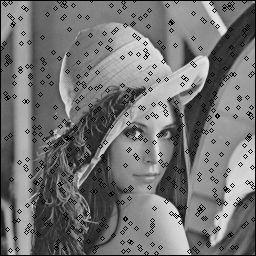
\includegraphics[width=\textwidth]{IMG/RandomInit/Initialization}
                \caption{Ants init positions}
                \label{fig:rand_init}
        \end{subfigure}%
        \qquad
        \begin{subfigure}[b]{0.3\textwidth}
                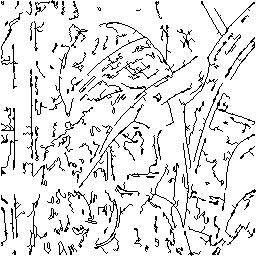
\includegraphics[width=\textwidth]{IMG/RandomInit/Iteration1}
                \caption{Iteration 1}
                \label{fig:rand_iter1}
        \end{subfigure}
        
        \vspace{5mm}
        
        \begin{subfigure}[b]{0.3\textwidth}
                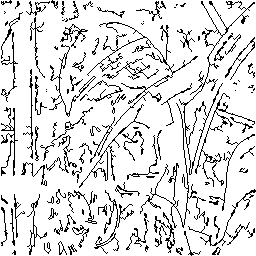
\includegraphics[width=\textwidth]{IMG/RandomInit/Iteration2}
                \caption{Iteration 2}
                \label{fig:rand_iter2}
        \end{subfigure}%
        \quad
        \begin{subfigure}[b]{0.3\textwidth}
                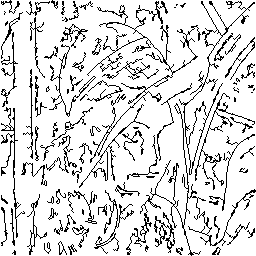
\includegraphics[width=\textwidth]{IMG/RandomInit/Iteration3}
                \caption{Iteration 3}
                \label{fig:rand_iter3}
        \end{subfigure}
        \quad
        \begin{subfigure}[b]{0.3\textwidth}
                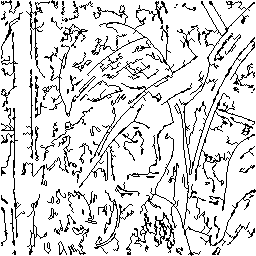
\includegraphics[width=\textwidth]{IMG/RandomInit/Iteration4}
                \caption{Iteration 4}
                \label{fig:rand_iter4}
        \end{subfigure}
        
        \vspace{5mm}
        
        \begin{subfigure}[b]{0.3\textwidth}
                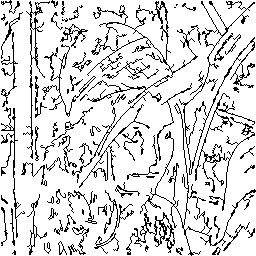
\includegraphics[width=\textwidth]{IMG/RandomInit/Iteration5}
                \caption{Iteration 5}
                \label{fig:rand_iter5}
        \end{subfigure}%
        \quad
        \begin{subfigure}[b]{0.3\textwidth}
                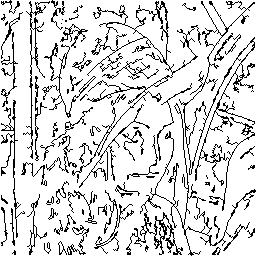
\includegraphics[width=\textwidth]{IMG/RandomInit/Iteration6}
                \caption{Iteration 6}
                \label{fig:rand_iter6}
        \end{subfigure}
        \quad
        \begin{subfigure}[b]{0.3\textwidth}
                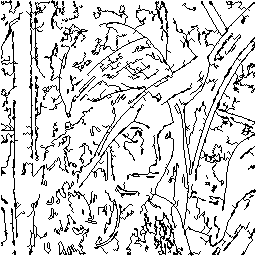
\includegraphics[width=\textwidth]{IMG/RandomInit/Iteration7}
                \caption{Iteration 7}
                \label{fig:rand_iter7}
        \end{subfigure}
        
        \vspace{5mm}
        
        \begin{subfigure}[b]{0.3\textwidth}
                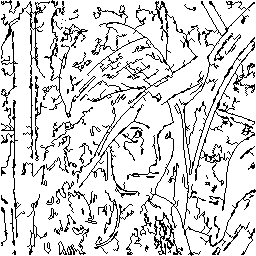
\includegraphics[width=\textwidth]{IMG/RandomInit/Iteration8}
                \caption{Iteration 8}
                \label{fig:rand_iter8}
        \end{subfigure}
        \quad
        \begin{subfigure}[b]{0.3\textwidth}
                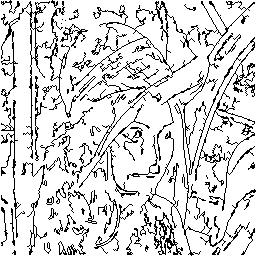
\includegraphics[width=\textwidth]{IMG/RandomInit/Iteration9}
                \caption{Iteration 9}
                \label{fig:rand_iter9}
        \end{subfigure}
        \quad
        \begin{subfigure}[b]{0.3\textwidth}
                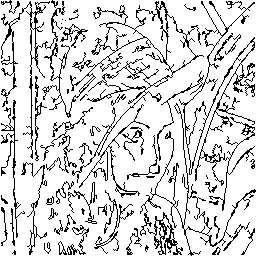
\includegraphics[width=\textwidth]{IMG/RandomInit/Iteration10}
                \caption{Iteration 10}
                \label{fig:rand_iter10}
        \end{subfigure}
        \caption{Ants are (a) initialized on random positions and (b)-(k) results are shown after each iteration is finished.}\label{fig:rand_init_approach}
	\end{figure}
	
	\section{Improving Search} \label{sec:imp_search}
	A good set of parameters for edge detection using ACS is presented in literature \cite{Anna:2010} by varying $q_0$ valie. The same set of parameter values are used for all the experiments proposed in this paper by fixing the value of $q_0$ to 0.7. Standard test image, Lena of size $256\times256$ is used to test the experiments. The value of each parameter is as follows:
	
	% Parameters
	\begin{itemize}
		\item Initial pheromone value ($\tau_{0}$) = 0.1
		\item Number of ants ($K$) = 512
		\item Number of iterations ($N$) = 10
		\item Number of constructions ($L$) = 40
		\item Parameter influencing pheromone trail ($\alpha$) = 1 (fixed to 1 for ACS)
		\item Parameter influencing heuristic information ($\beta$) = 1
		\item Pheromone decay coefficient ($\varphi$) = 0.05 (used for local pheromone update)
		\item Pheromone evaporation coefficient ($\rho$) = 0.1 (used for global pheromone update)
		\item Degree of exploration ($q_{0}$) = 0.7
	\end{itemize}
	
	% Init ants on heuristics
	\subsection{Initialize Ants on Better Heuristics}\label{subsec:init_ants}
	Most of the literature including \cite{Manish:2013,Jian:2012} concentrate on improving the heuristic. The proposed technique try to improve the search instead, to best fit for the image edge detection. The biggest disadventage of initializing ants on random positions is, it leaves noise on the image, and even the theresholding technique to remove noise may remove some important details on the edges. Removing noise means, the work done by most of the ants is simply wasted. Since, the heuristic matrix for the entire image could be constructed before starting the algorithm, it is easier to guide all the ants to start at good locations where most of the solutions produced by ants could be used without thresholding.
	
	%FIGURE: Heuristic Initialization
	\begin{figure}
        \centering
        \begin{subfigure}[b]{0.3\textwidth}
                \includegraphics[width=\textwidth]{IMG/HeuristicInit/Initialization}
                \caption{Ants init positions}
                \label{fig:heu_init}
        \end{subfigure}%
        \qquad
        \begin{subfigure}[b]{0.3\textwidth}
                \includegraphics[width=\textwidth]{IMG/HeuristicInit/Iteration1}
                \caption{Iteration 1}
                \label{fig:heu_iter1}
        \end{subfigure}
        
        \vspace{5mm}
        
        \begin{subfigure}[b]{0.3\textwidth}
                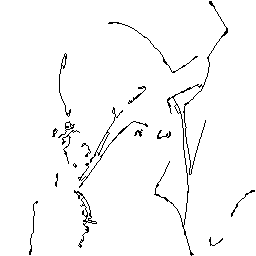
\includegraphics[width=\textwidth]{IMG/HeuristicInit/Iteration2}
                \caption{Iteration 2}
                \label{fig:heu_iter2}
        \end{subfigure}%
        \quad
        \begin{subfigure}[b]{0.3\textwidth}
                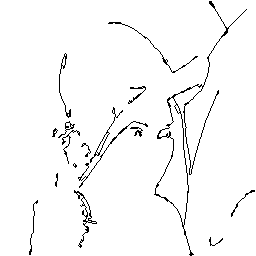
\includegraphics[width=\textwidth]{IMG/HeuristicInit/Iteration3}
                \caption{Iteration 3}
                \label{fig:heu_iter3}
        \end{subfigure}
        \quad
        \begin{subfigure}[b]{0.3\textwidth}
                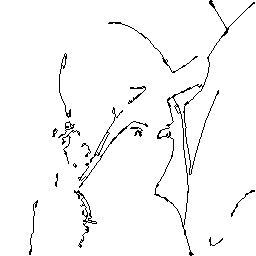
\includegraphics[width=\textwidth]{IMG/HeuristicInit/Iteration4}
                \caption{Iteration 4}
                \label{fig:heu_iter4}
        \end{subfigure}
        
        \vspace{5mm}
        
        \begin{subfigure}[b]{0.3\textwidth}
                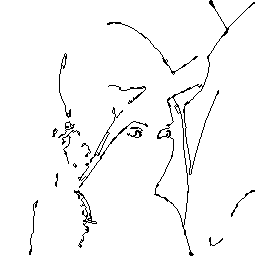
\includegraphics[width=\textwidth]{IMG/HeuristicInit/Iteration5}
                \caption{Iteration 5}
                \label{fig:heu_iter5}
        \end{subfigure}%
        \quad
        \begin{subfigure}[b]{0.3\textwidth}
                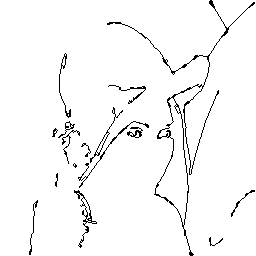
\includegraphics[width=\textwidth]{IMG/HeuristicInit/Iteration6}
                \caption{Iteration 6}
                \label{fig:heu_iter6}
        \end{subfigure}
        \quad
        \begin{subfigure}[b]{0.3\textwidth}
                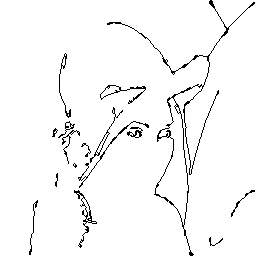
\includegraphics[width=\textwidth]{IMG/HeuristicInit/Iteration7}
                \caption{Iteration 7}
                \label{fig:heu_iter7}
        \end{subfigure}
        
        \vspace{5mm}
        
        \begin{subfigure}[b]{0.3\textwidth}
                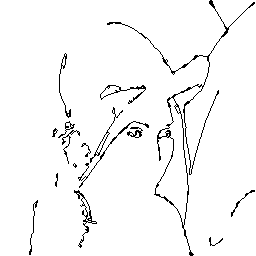
\includegraphics[width=\textwidth]{IMG/HeuristicInit/Iteration8}
                \caption{Iteration 8}
                \label{fig:heu_iter8}
        \end{subfigure}
        \quad
        \begin{subfigure}[b]{0.3\textwidth}
                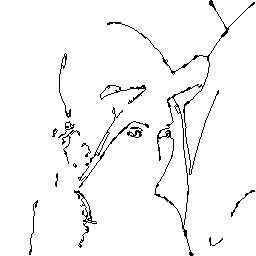
\includegraphics[width=\textwidth]{IMG/HeuristicInit/Iteration9}
                \caption{Iteration 9}
                \label{fig:heu_iter9}
        \end{subfigure}
        \quad
        \begin{subfigure}[b]{0.3\textwidth}
                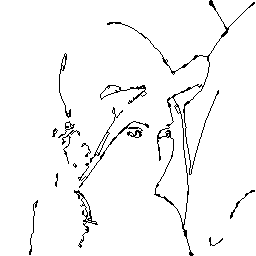
\includegraphics[width=\textwidth]{IMG/HeuristicInit/Iteration10}
                \caption{Iteration 10}
                \label{fig:heu_iter10}
        \end{subfigure}
        \caption{Ants are (a) initialized on positions where heuristic values are high and (b)-(k) results are shown after each iteration is finished.}\label{fig:heuristic_approach}
	\end{figure}

	% Improved search
	\subsection{Reinitialize Ants Based on Performance}\label{subsec:improve_search}
	Initializing ants on best heuristic positions has shown a drastic improvement over the method that initializes the ants on random positions. However, after certain iterations the result stagnates. Consequently, the ants may not find the remaining possible edges. Therefore, this experiment extends the previous one by adding an initialization step after each iteration. 
	
	On each iteration, the amount of pheromone deposited by each ant at local and global pheromone deposit steps are maintained. After global pheromone deposit (step 7 in algorithm \ref{alg:aco}) the average amount of pheromone ($\tau_{avg}$) deposited by all the ants is calculated. Before starting the next iteration, the ants which deposit the pheromone less than the avarage amount ($\tau_{avg}$) calculated are reinitialized to the next heighest heuristic position and the ant's memory of positions visited in the past is reset. Thus, the ants which performed above the average are left on their latest location to find the connected edges. The ants which performed below the average assume that there are no connected edges to find and move to new positions to find further possible edges. The result after each iteration is as shown in figure \ref{fig:search_improved}. The results show that, this method tends to find edges at other positions without loosing most of the edges found so far. Comparision of three experiments made in this paper is presented in next section.
		
	%FIGURE: Improved Search
	\begin{figure}
        \centering
        \begin{subfigure}[b]{0.3\textwidth}
                \includegraphics[width=\textwidth]{IMG/ImprovedSearch/Initialization}
                \caption{Ants init positions}
                \label{fig:search_init}
        \end{subfigure}%
        \qquad
        \begin{subfigure}[b]{0.3\textwidth}
                \includegraphics[width=\textwidth]{IMG/ImprovedSearch/Iteration1}
                \caption{Iteration 1}
                \label{fig:search_iter1}
        \end{subfigure}
        
        \vspace{5mm}
        
        \begin{subfigure}[b]{0.3\textwidth}
                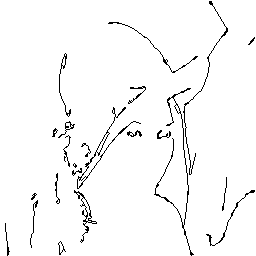
\includegraphics[width=\textwidth]{IMG/ImprovedSearch/Iteration2}
                \caption{Iteration 2}
                \label{fig:search_iter2}
        \end{subfigure}%
        \quad
        \begin{subfigure}[b]{0.3\textwidth}
                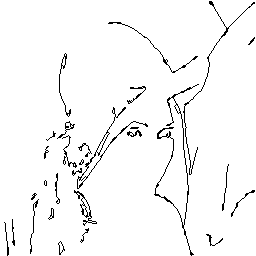
\includegraphics[width=\textwidth]{IMG/ImprovedSearch/Iteration3}
                \caption{Iteration 3}
                \label{fig:search_iter3}
        \end{subfigure}
        \quad
        \begin{subfigure}[b]{0.3\textwidth}
                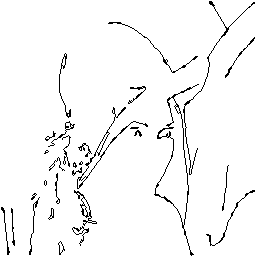
\includegraphics[width=\textwidth]{IMG/ImprovedSearch/Iteration4}
                \caption{Iteration 4}
                \label{fig:search_iter4}
        \end{subfigure}
        
        \vspace{5mm}
        
        \begin{subfigure}[b]{0.3\textwidth}
                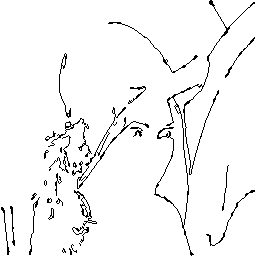
\includegraphics[width=\textwidth]{IMG/ImprovedSearch/Iteration5}
                \caption{Iteration 5}
                \label{fig:search_iter5}
        \end{subfigure}%
        \quad
        \begin{subfigure}[b]{0.3\textwidth}
                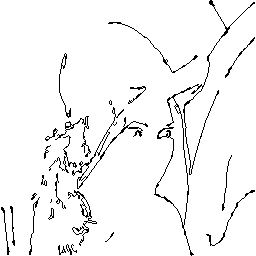
\includegraphics[width=\textwidth]{IMG/ImprovedSearch/Iteration6}
                \caption{Iteration 6}
                \label{fig:search_iter6}
        \end{subfigure}
        \quad
        \begin{subfigure}[b]{0.3\textwidth}
                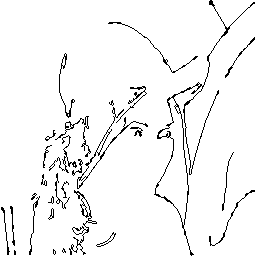
\includegraphics[width=\textwidth]{IMG/ImprovedSearch/Iteration7}
                \caption{Iteration 7}
                \label{fig:search_iter7}
        \end{subfigure}
        
        \vspace{5mm}
        
        \begin{subfigure}[b]{0.3\textwidth}
                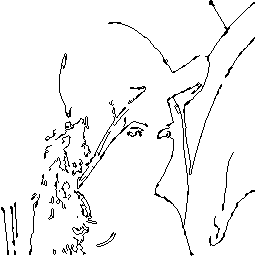
\includegraphics[width=\textwidth]{IMG/ImprovedSearch/Iteration8}
                \caption{Iteration 8}
                \label{fig:search_iter8}
        \end{subfigure}
        \quad
        \begin{subfigure}[b]{0.3\textwidth}
                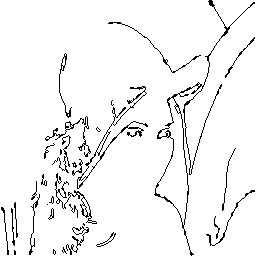
\includegraphics[width=\textwidth]{IMG/ImprovedSearch/Iteration9}
                \caption{Iteration 9}
                \label{fig:search_iter9}
        \end{subfigure}
        \quad
        \begin{subfigure}[b]{0.3\textwidth}
                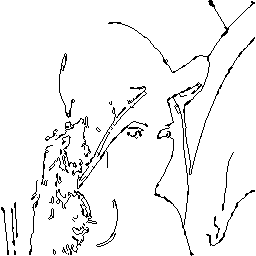
\includegraphics[width=\textwidth]{IMG/ImprovedSearch/Iteration10}
                \caption{Iteration 10}
                \label{fig:search_iter10}
        \end{subfigure}
        \caption{Ants are (a) initialized on positions where heuristic values are high and (b)-(k) after each iteration ants pheromone deposit below the average are reinitialized and results are shown.}\label{fig:search_improved}
	\end{figure}
	
	The best heuristic depends on the nature of task. For edge detection using ACS, the best heuristics are the positions where the heuristic values are high. Therefore, $K$ ants are initialized on $K$ positions in decreasing order of heuristic values as part of ACS, and the results after each iteration are as shown in figure \ref{fig:heuristic_approach}. The binary image after ecah iteration is presented and no thresholding is applied. Thre results show that, all the edges found by ants are potential edges and there is a great performance improvement compared to previous method (random initialization), because no ant's effort is wasted. After few iterations, the results will not be improved (stagnation) as shown in figure \ref{fig:heu_iter8} - \ref{fig:heu_iter10}, there is no much difference bwteen images means that all the ants move on previously visited positions (by any ant) without finding further possible edges. Section \ref{subsec:improve_search} proposes a technique to solve the stagnation, and improves the search to find further possible edges.
	
	
	%Comparision
	\section{Analysis of Results}\label{sec:comparision}
	The amount of pheromone deposited by each ant on each iteration is maintained, and the average of pheromone deposit on each iteration is plotted as shown in figure \ref{fig:avg_plot}. For all the three experiments made, box plot for the ants pheromone deposit in each method on each iteration is plotted as in figure \ref{fig:box_plt}. Initializing ants on random positions shows poor performance over the other two methods as the avrage pheromone deposit is too low on each iteration.
	
	%FIGURE: Image Graph
	\begin{figure}[H]
		\centering
		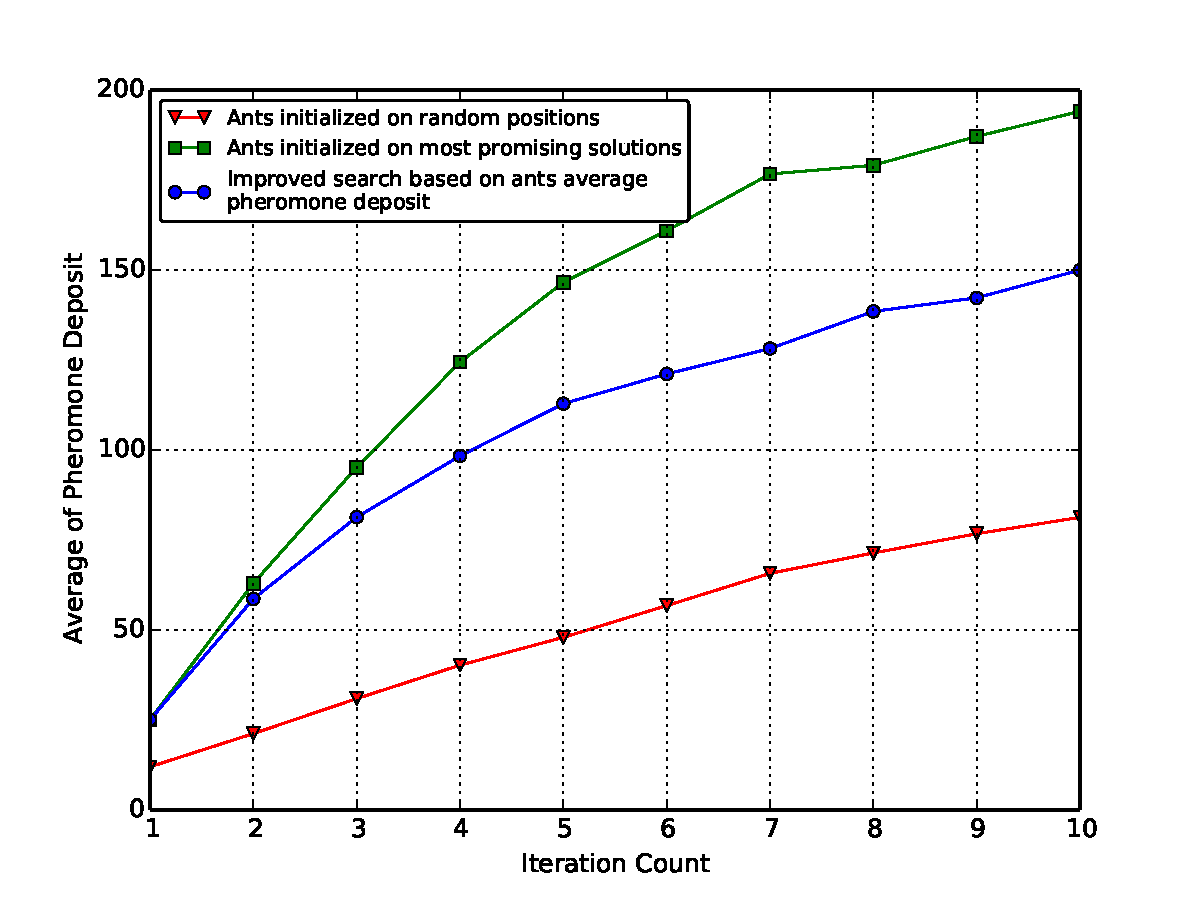
\includegraphics[width=0.92\textwidth]{PLT/Comparision/average}
		\caption{Plot showing the average amount of pheromone deposited by all the ants on each iteration.}
		\label{fig:avg_plot}
	\end{figure}
	
	
	%FIGURE: Comparision
	\begin{figure}[H]
        \centering
        \begin{subfigure}[b]{0.3\textwidth}
                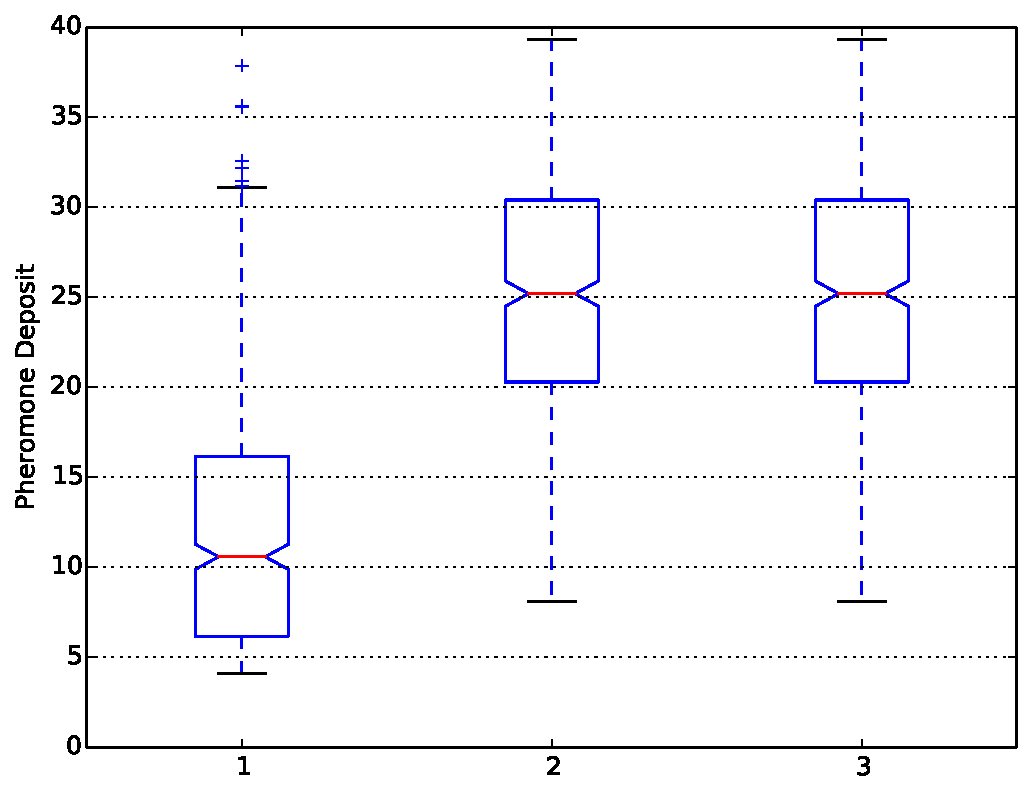
\includegraphics[width=\textwidth]{PLT/Comparision/BOXPLOT/Iteration1}
                \caption{Iteration 1}
                \label{fig:plt_iter1}
        \end{subfigure}
        
        \begin{subfigure}[b]{0.3\textwidth}
                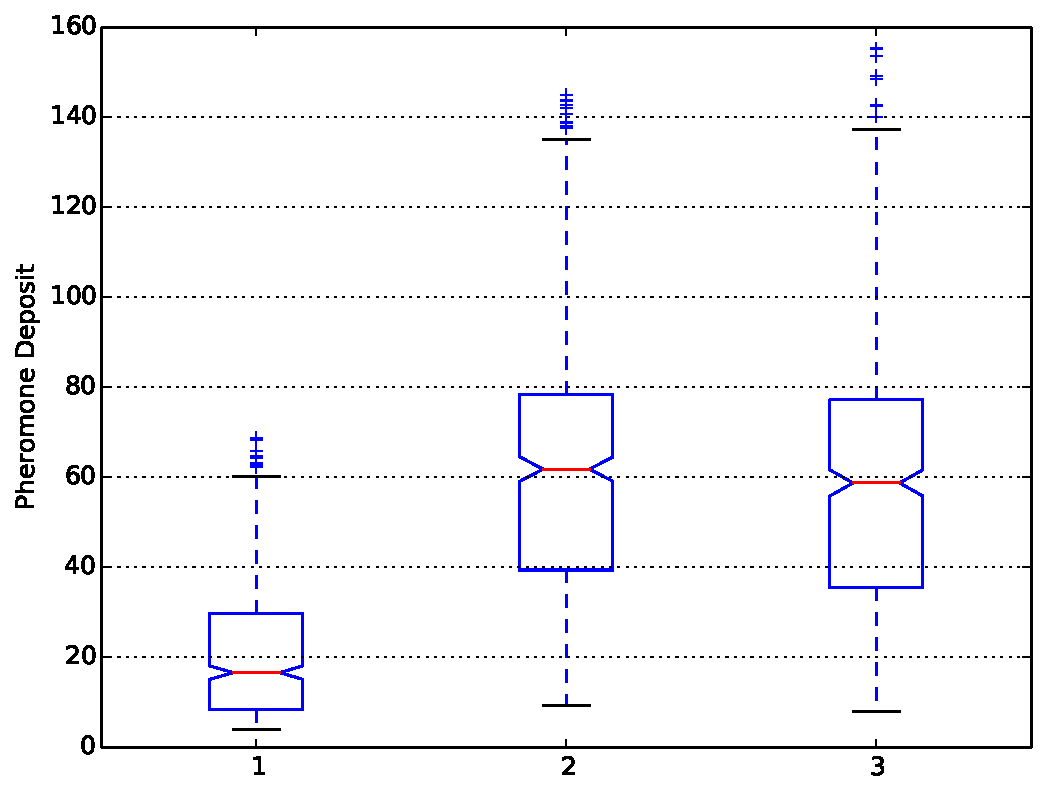
\includegraphics[width=\textwidth]{PLT/Comparision/BOXPLOT/Iteration2}
                \caption{Iteration 2}
                \label{fig:plt_iter2}
        \end{subfigure}%
        \quad
        \begin{subfigure}[b]{0.3\textwidth}
                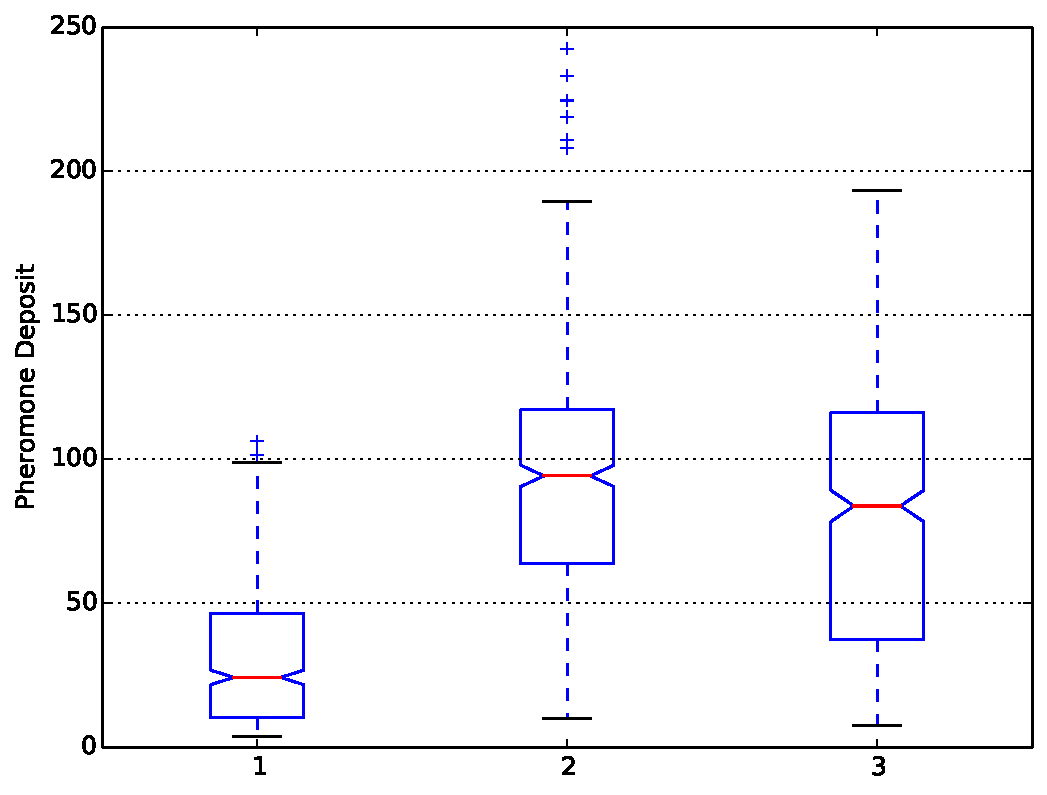
\includegraphics[width=\textwidth]{PLT/Comparision/BOXPLOT/Iteration3}
                \caption{Iteration 3}
                \label{fig:plt_iter3}
        \end{subfigure}
        \quad
        \begin{subfigure}[b]{0.3\textwidth}
                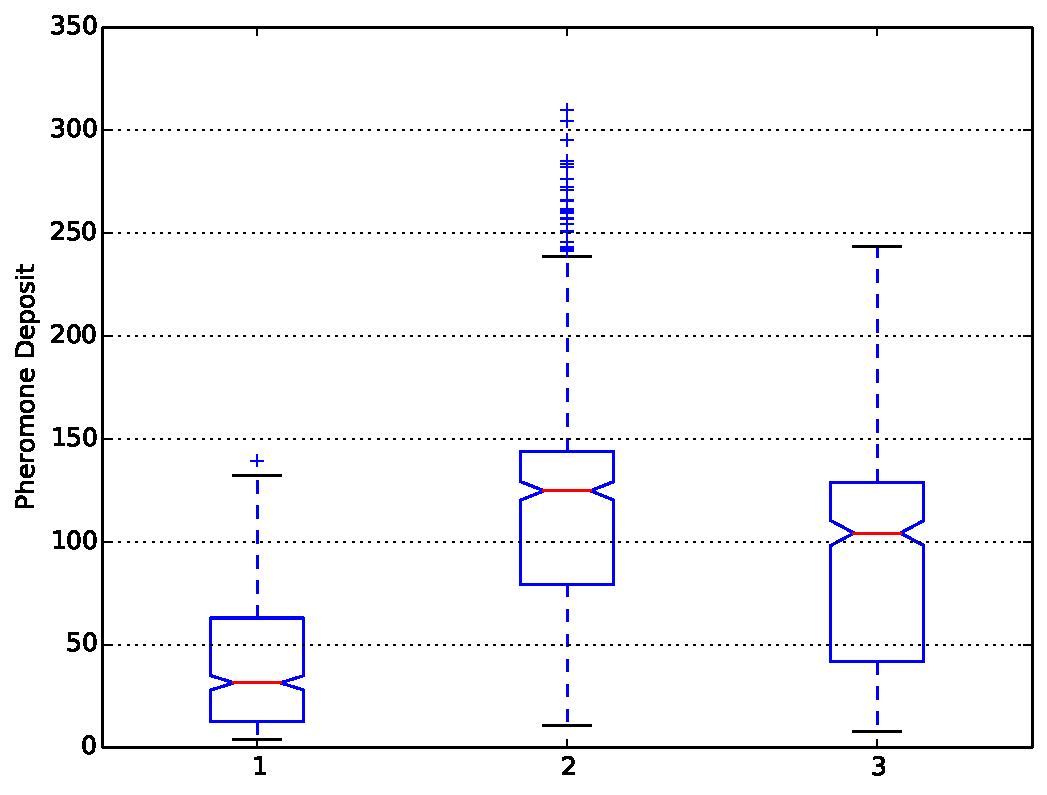
\includegraphics[width=\textwidth]{PLT/Comparision/BOXPLOT/Iteration4}
                \caption{Iteration 4}
                \label{fig:plt_iter4}
        \end{subfigure}
        
        \vspace{5mm}
        
        \begin{subfigure}[b]{0.3\textwidth}
                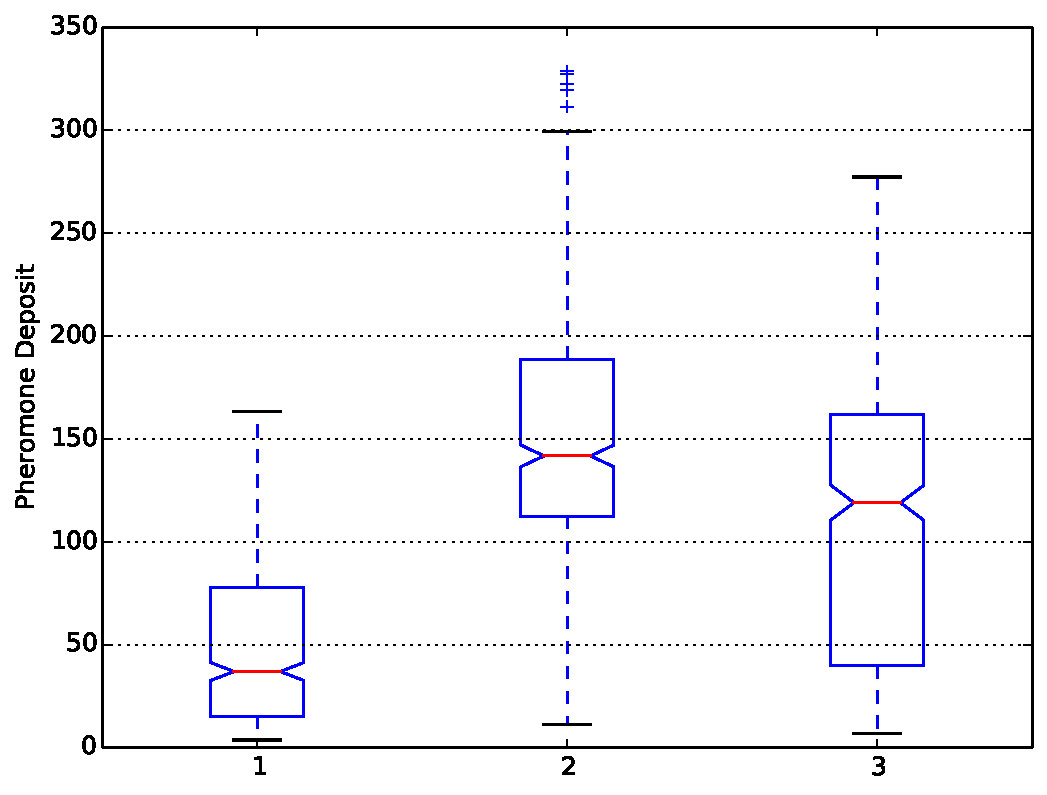
\includegraphics[width=\textwidth]{PLT/Comparision/BOXPLOT/Iteration5}
                \caption{Iteration 5}
                \label{fig:plt_iter5}
        \end{subfigure}%
        \quad
        \begin{subfigure}[b]{0.3\textwidth}
                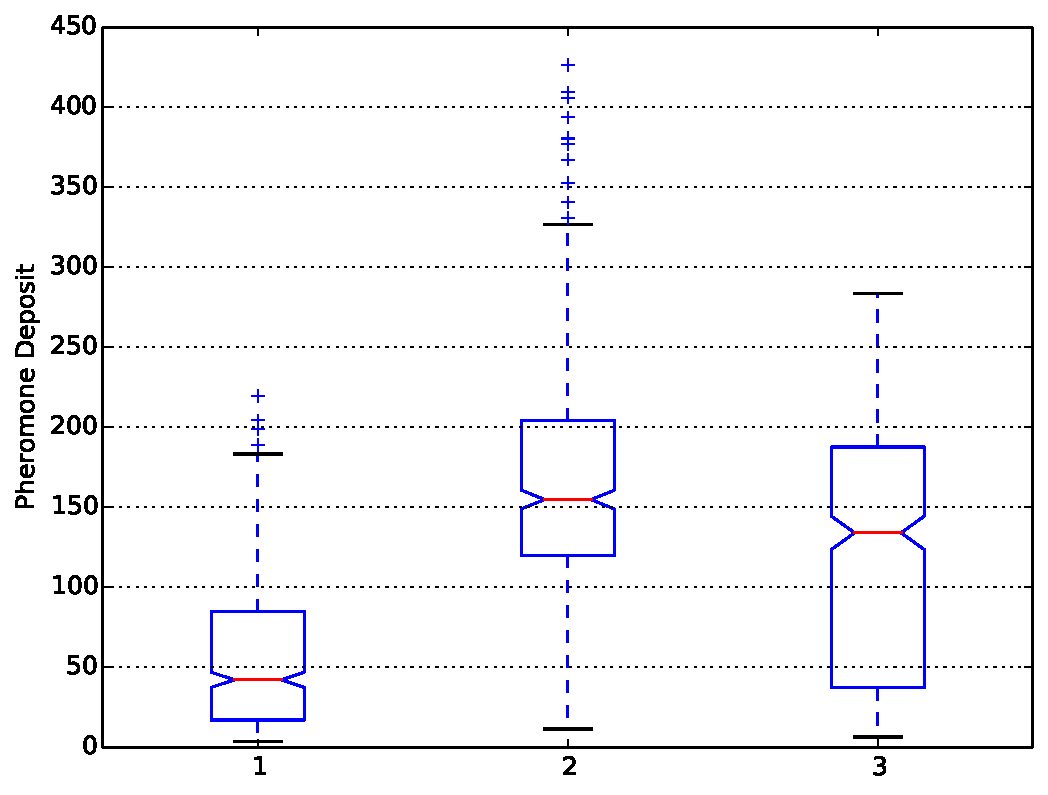
\includegraphics[width=\textwidth]{PLT/Comparision/BOXPLOT/Iteration6}
                \caption{Iteration 6}
                \label{fig:plt_iter6}
        \end{subfigure}
        \quad
        \begin{subfigure}[b]{0.3\textwidth}
                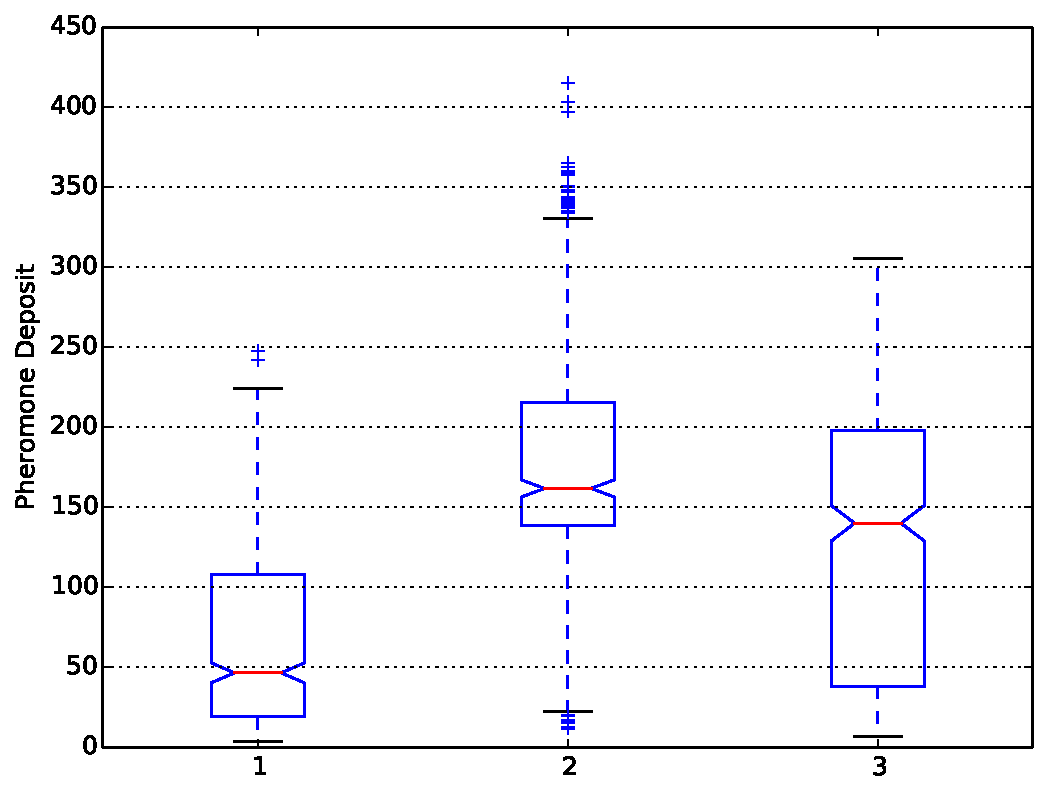
\includegraphics[width=\textwidth]{PLT/Comparision/BOXPLOT/Iteration7}
                \caption{Iteration 7}
                \label{fig:plt_iter7}
        \end{subfigure}
        
        \vspace{5mm}
        
        \begin{subfigure}[b]{0.3\textwidth}
                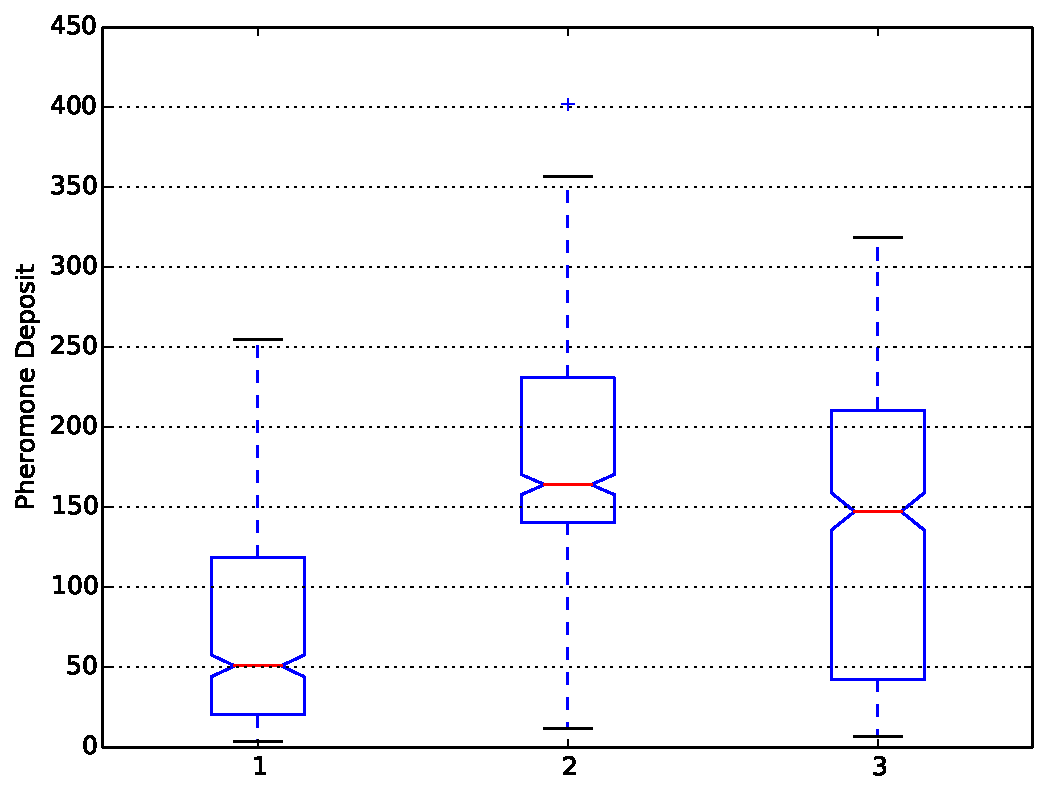
\includegraphics[width=\textwidth]{PLT/Comparision/BOXPLOT/Iteration8}
                \caption{Iteration 8}
                \label{fig:plt_iter8}
        \end{subfigure}
        \quad
        \begin{subfigure}[b]{0.3\textwidth}
                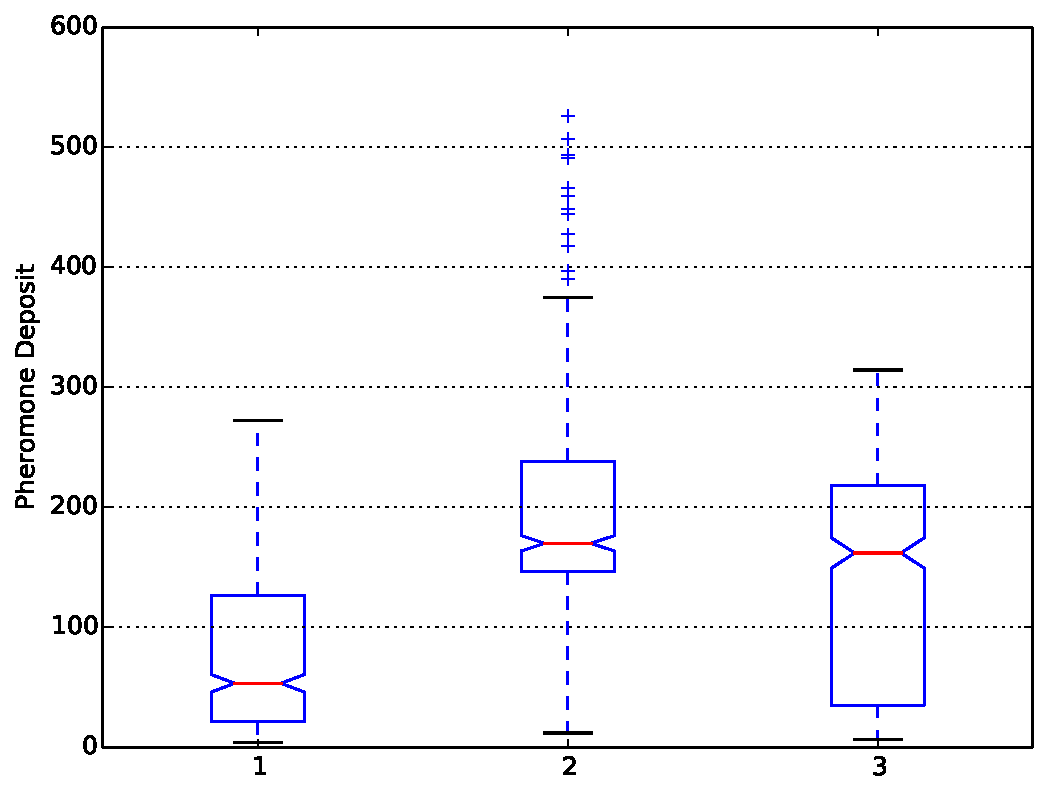
\includegraphics[width=\textwidth]{PLT/Comparision/BOXPLOT/Iteration9}
                \caption{Iteration 9}
                \label{fig:plt_iter9}
        \end{subfigure}
        \quad
        \begin{subfigure}[b]{0.3\textwidth}
                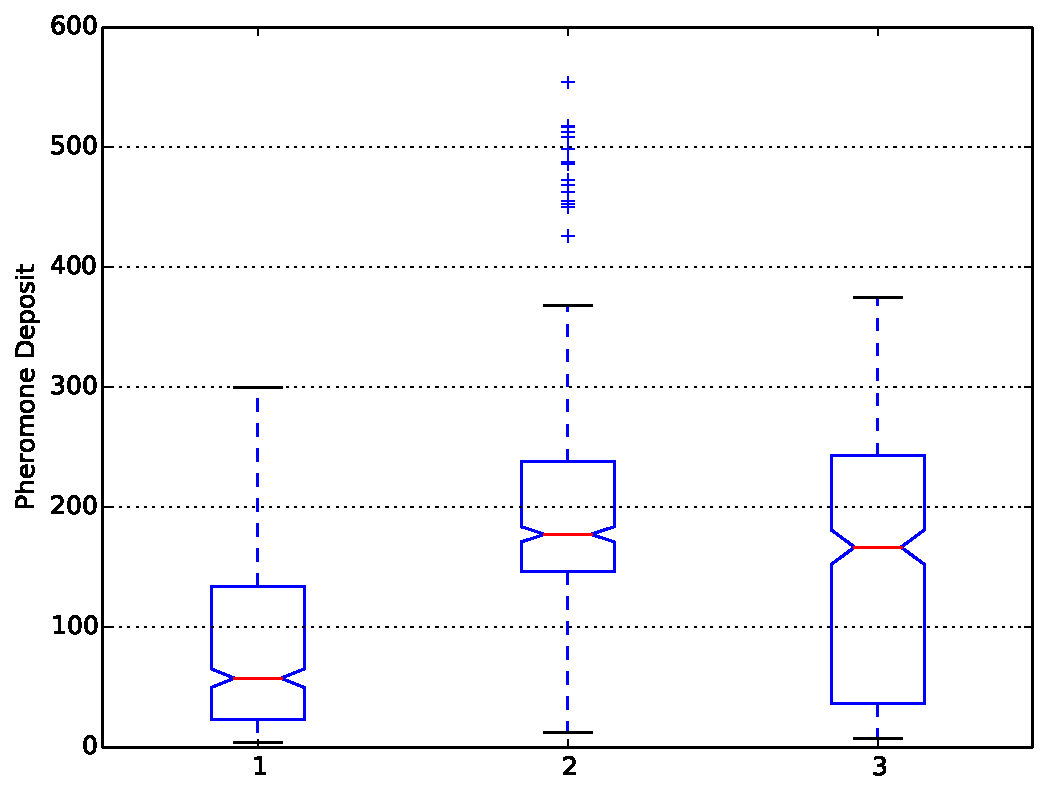
\includegraphics[width=\textwidth]{PLT/Comparision/BOXPLOT/Iteration10}
                \caption{Iteration 10}
                \label{fig:plt_iter10}
        \end{subfigure}
        \caption{Box plot for pheromone deposit by each ant on each iteration for three methods, (1) Ants initialized on random positions, (2) ants initialized on positions where heuristic values are high, and (3) reinitialize ants after each iteration based on their average performance.}\label{fig:box_plt}
	\end{figure}
	
	Although, the second approach, the method that initializes ants on better heuristics has more average pheromone deposit on each iteration, the outliers above the upper whisker in boxplot (position 2 on X-axis in figure \ref{fig:box_plt}) prove that the ants deposited large amount of pheromone have influenced the average value, and ants try to move towards the best solutions already found rather than finding other possibilities. Third approach, reinitialize ants below the average performance, (position 3 on X-axis in figure \ref{fig:box_plt}) the wide spread of inter quartile range (IQR) shows that the ants pheromone deposit is more deviated which means, several ants try to find new edges on each iteration.
	
	%Conclusion
	\section{Conclusion}\label{sec:conclusion}
	Reassigning ants below the average performance has excelled, because the result never gets stagnated. Especially, when the image has more disconnected edges (for example, the hair part on the test image), this method eventually finds all the edges. There is a possibility that the edges found during early iterations may disappear in the later because of pheromone evaporation. But, blending all the results after each iteration would give the complete possible edges. A simple heuristic is used for the experiments made in this paper. Improving heuristic and hybridization on top of the proposed method may further improve the solutions.
	
	
	
	\bibliographystyle{splncs}
	\bibliography{literature}
	\nocite{*}
	
\end{document}